\documentclass[10pt,a4paper]{article}
\usepackage[utf8]{inputenc}

% \usepackage{ngerman}  % german documents
\usepackage{graphicx}  % import graphics einbinden
\usepackage{listings}  % support source code listing
\usepackage{amsmath}  % math stuff
\usepackage{amssymb} % 
\usepackage{a4wide} % wide pages
\usepackage{fancyhdr} % nice headers
\lstset{basicstyle=\footnotesize,language=Python,numbers=left, numberstyle=\tiny, stepnumber=5,firstnumber=0, numbersep=5pt} % set up listings
\pagestyle{fancy}             % header
\setlength{\parindent}{0pt}   % no indentation

\usepackage[pdfpagemode=None, colorlinks=true,  % url coloring
           linkcolor=blue, urlcolor=blue, citecolor=blue, plainpages=false, 
           pdfpagelabels,unicode]{hyperref}
           
% change enums style: first level (a), (b), (c)           
\renewcommand{\labelenumi}{(\alph{enumi})}
\renewcommand{\labelenumii}{(\arabic{enumii})}

%lecture name
\newcommand{\lecture}{
	Bioinformatics III
}           

%assignment iteration
\newcommand{\assignment}{
	First Assignment
}

%set up names, matricle number, and email
\newcommand{\authors}{
  \begin{tabular}{rl}
    \href{mailto:s9alfloh@stud.uni-saarland.de}{Alexander Flohr} & (2549738)\\
    \href{mailto:s9ankupi@stud.uni-saarland.de}{Andrea Kupitz} & (2550260)
  \end{tabular}
}

% use to start a new exercise
\newcommand{\exercise}[1]
{
  \stepcounter{subsection}
  \subsection*{Exercise \thesubsection: #1}

}

\begin{document}
\title{\Large \lecture \\ \textbf{\normalsize \assignment}}
\author{\authors}

\setlength \headheight{25pt}
\fancyhead[R]{\begin{tabular}{r}\lecture \\ \assignment \end{tabular}}
\fancyhead[L]{\authors}


\setcounter{section}{1} % modify for later sheets, i.e. 2, 3, ...
%\section{Introduction to Python and some Network Properties} % optional, note that section invocation sets the section counter + 1, so adapt the setcounter command
\maketitle

\exercise{The random network}
\begin{enumerate}
\item Listing \ref{ex1-1} shows source code.
\lstinputlisting[label=ex1-1,caption={Example Listing of source code}] {Node.py}

\item Listing \ref{ex1-2} shows source code.
\lstinputlisting[label=ex1-2,caption={Example Listing of source code}] {AbstractNetwork.py}

\item Listing \ref{ex1-3} shows source code.
\lstinputlisting[label=ex1-3,caption={Example Listing of source code}] {RandomNetwork.py}
\end{enumerate}

\exercise{Degree Distribution}
\begin{enumerate}
\item Listing \ref{ex2-1} shows source code.
\lstinputlisting[label=ex2-1,caption={Example Listing of source code}] {DegreeDistribution.py}

\item Listing \ref{ex2-2} shows source code.
\lstinputlisting[label=ex2-2,caption={Example Listing of source code}] {Tools.py}
\textbf{{"}Why does this happen and how do you need to ”fill” the shorter distributions?{"}}\\
Our network distribution is designed to be as long as the maximal node degree. If the links are distributed perfectly, our distribution would always be $\lambda$ long. Unfortunately, this is very unlikely. In the worst case, all links could be attached to one node, increasing the number of distribution entities up to the number of links. Furthermore, every distribution differing from the perfect one causes variances in the length of the degree distribution.\\
Additionally, the user defines the length of the entities calculated for the poisson distribution. Therefore, different length in the data can occure.\\
Extensions of the random network derived data can be done by appending the required amount of zeros without disrupting the reults.\\
The same can be done for the poisson distributed data, but it is not possible to keep the distribution if the distribution is only given for the first couple of entities.\\
\textbf{Are the ranges of the discrete distributions we obtain in (c) deterministic in our case?}\\
To answere this question, we first look at the definition of deterministic systems. {"}\textit{ In mathematics, computer science and physics, a deterministic system is a system in which no randomness is involved in the development of future states of the system. A deterministic model will thus always produce the same output from a given starting condition or initial state.}{"} (see Wikipedia artice of deterministic systems, \url{https://en.wikipedia.org/wiki/Deterministic_system}. With this knowledge, it is easy to show, that plot 1 is not deterministic, because further runs always produce new results. The same can be sad about the second plot, even if the changes are nearly invisible, the created random networks are allways different. Therefore, the plots ranges of the discrete distribution are not deterministic.\\
But: The curves representing the poisson distribution are dterministic, because the distribution will not change if the input parameters remain the same.
\item Listing \ref{ex2-3} shows source code.
\lstinputlisting[label=ex2-3,caption={Example Listing of source code}] {createAndPlotNetworks.py}
This script resulted in figure \ref{ex2-p1} and \ref{ex2-p2}.

\begin{figure}[!h]
  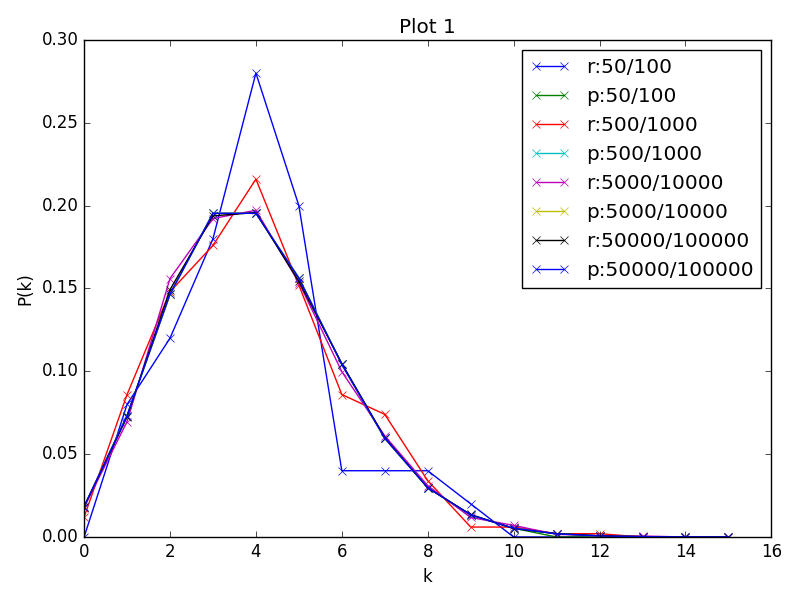
\includegraphics[width=\linewidth]{Plot_1.png}
  \caption{Plot 1. Setup provided in Listing \ref{ex2-3}}
  \label{ex2-p1}
\end{figure}
\begin{figure}[h]
  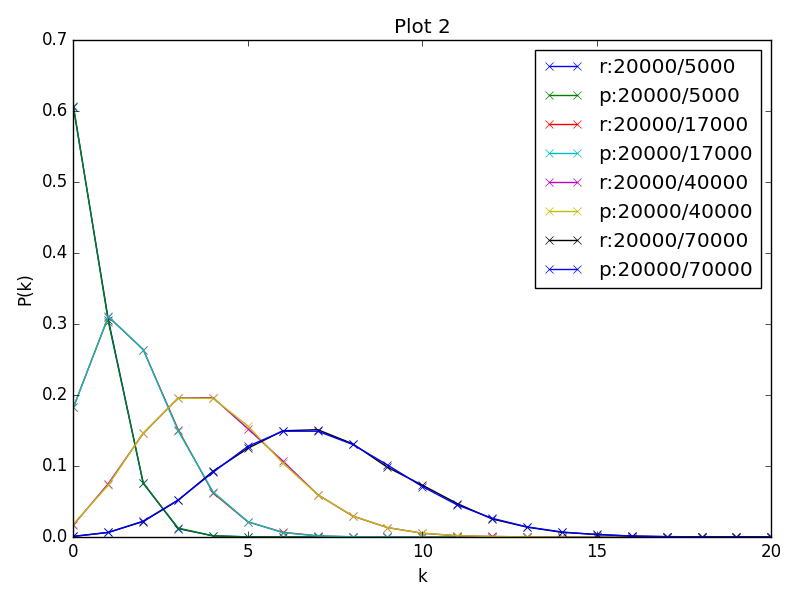
\includegraphics[width=\linewidth]{Plot_2.png}
  \caption{Plot 1. Setup provided in Listing \ref{ex2-3}}
  \label{ex2-p2}
\end{figure}

Both figure \ref{ex2-p1} and \ref{ex2-p2} show the degree distribution of different random networks. Thereby, lines listed in the legend starting with a {"}r{"} represent raw data, obtained by a randomly generated network. Their code is shown in listing \ref{ex1-3}. The distribution evaluation code can be found in listing\ref{ex2-1}. Curves with names starting on {"}p{"} are created with the code, provided in listing \ref{ex2-2} and represent the poisson distribution.\\
The network setup for plot \ref{ex2-p1} consists of random network with twice as many links as nodes. Since, every link attaches two nodes, we can expect every node to have an average degree of 4. Therefore, the expectation value $\lambda$ is determined to be 4. Due to this circumstance, the {"}p{"} lines have 100{\%} overlap. The degree distribution created by our random networks follows the same distribution. Further observable is that by increasing the number of nodes and edges, we converge with the poisson distribution.\\
For plot \ref{ex2-p2}, we first concentrate on the estimated poisson distributions:\\
\begin{table}
	\caption{Expected $\lambda$}
	\label{ex2-lambda}
	\begin{tabular}{|r|r|c|}
	\hline 
	Nodes & Links & $\lambda$\\
	\hline \hline
	20000 & 5000 & 0.5\\
	\hline
	20000 & 17000 & 1.7\\
	\hline
	20000 & 40000 & 4\\
	\hline
	20000 & 70000 & 7\\
	\hline
	\end{tabular}
The $\lambda$ values are determined to be de twice the number of links divided by the number of nodes. As mentioned before, we concerge with the poisson distribution when increasing the number of nodes and links. Due to this, it is nearly impossible to distinguish between the last two (legend order) lines within the plot. The same holds true for all other pairs of lines.
\end{table}



\end{enumerate}
\end{document}